\chapter{Trennen}

\section{Stoffgemische}

%Tabelle START

\vspace*{-2.5mm}
\renewcommand{\arraystretch}{1.2}
\begin{table}[h!]
	\centering
	\caption{Stoffgemische}
	\label{tab:tabelle1}
	%\resizebox{10cm}{!}{
	\begin{tabulary}{\textwidth}{C|L}
		\hline
		\textbf{Kombination der Phasen} & \textbf{Bezeichnung}\\
		\hline
		S in G & Rauch, Staub,...\\
		S in L (Aerosol)& Suspension, Schlamm, Trübe,...\\
		L in G (Aerosol)& Dampfwolken, Nebel, Regen, Sprühwolke,...\\
		G in L & Sprudelschicht, Blasenschwarm, Schaum,...\\
		L in L & Emulsion, Tropfenschwarm\\
	\end{tabulary}
	%}
\end{table}
\FloatBarrier
\vspace*{-2.5mm}

%Tabelle Ende

\section{Trennverfahren}

Alle Stoffsysteme sind dispers und bestehen aus mindestens 2 Phasen.\\
Nur dann kann man \underline{mechanische Trennverfahren} anwenden. \\
(Grenze nach unten ist dabei die Partikelgröße)\\ \\
Für einphasige Stoffsysteme müssen thermische Trennverfahren angewendet werden.\\
Mechanische Verfahren sind meist effizienter als thermische Verfahren.

\begin{itemize}
	\item \textbf{Sedimentation} $\approx \SI{10}{\micro \meter}$ \begin{small}(S/G, S/L, L/L, G/L, L/G)\end{small}\\
	= Absetzen/Aufsteigen von Teilchen im Schwerkraftfeld \\ \\
	$\rightarrow$ \textit{Voraussetzung:} \\
	unterschiedliche Dichte der Teilchen gegenüber Fluid
		
	\item \textbf{Zentrifugation} $< \SI{10}{\micro \meter}$ \begin{small}(S/L)\end{small}\\
	= Trennen im Zentrifugalfeld \\ \\
	$\rightarrow$ geeignet für sehr geringe Dichteunterschiede und sehr kleine Teilchen
	
	\item \textbf{Filtration} \begin{small}(S/G, S/L)\end{small}\\
	= Teilchendurchmesser > Porendurchmesser des Filtermediums \\
	"`Sterische (räumliche) Hinderung"' 
	
	\item \textbf{Sieben} \begin{small}(S/G)\end{small}\\
	= Trennen nach Größenunterschied \\
	$\rightarrow$ Klassierung
	
	\item \textbf{Sichten} \begin{small}(S/G)\end{small}\\
	= Trennen nach Luftwiderstand und Dichte
	
	\item \textbf{Flotation} \begin{small}(S/S/G)\end{small}\\
	= spezielle Sedimentation
	
	\item \textbf{Zyklon} \begin{small}(S/G, S/L)\end{small}\\
	= ähnlich wie Zentrifugation
\end{itemize}

\subsection{Sedimentation}
= Absetzen einer dispersen Phase unter Einwirkung der Schwerkraft\\

Disperse Phase kann eine höhere oder niedrigere Dichte haben, als die Kontinuierliche.\\
$\rightarrow$ wichtige Trennoperation, weil Apparate \underline{einfach} und somit \underline{günstig} sind\\

\textbf{Bezeichnung des Sediments nach Zweck}
\begin{itemize}
	\item \textit{Klären:} \\
	Trennziel = klare Flüssigkeit mit möglichst wenig Teilchen
	\item \textit{Eindicken:} \\
	Trennziel = möglichst konzentrierter Schlamm mit möglichst wenig Flüssigkeit
\end{itemize}



\newpage

\section{Grundlagen der Modellierung}
Bewegung eines Einzelteilchens im Schwerkraftfeld\\
$\rightarrow$ Annahme: Teilchen ist starr, kugelförmig und glatt\\ \\
$d_P>\SI{10}{\micro \meter}$\\
$\rho_P>\rho_F$
\vspace*{-20mm}
%Start
\begin{figure}[h!]
	\centering
	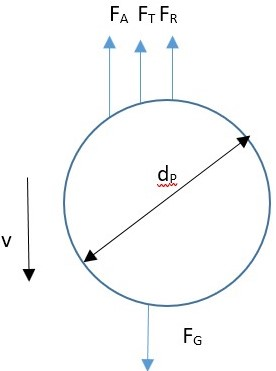
\includegraphics[width=0.22\textwidth]{img/partikelmodell}
	\caption{Skizze eines Partikels}
	\label{skizzepruef}
\end{figure}
\FloatBarrier
%Ende
\vspace*{-5mm}
\begin{flalign}
F_G &= m_P*g=V_P*\rho_P*g=\frac{\pi}{6}*d_P^3*\rho_P*g\\
F_T &= m_F*g=V_P*\rho_F*g=\frac{\pi}{6}*d_P^3*\rho_F*g
\end{flalign}
\begin{small}\begin{center}"'Auftrieb ist Masse der verdrängten Flüssigkeit"'\end{center}\end{small}
\vspace*{-5mm}
\begin{flalign}
F_R &= c_W*\rho_F*\frac{1}{2}*v_P^2*A_\perp
\end{flalign}


$c_W$... Widerstandsbeiwert $c_W=f(v,\text{Geometrie}, \text{Rauigkeit},...)$\\
$v_P$... Relativgeschwindigkeit zwischen Teilchen und Partikel\\
$A_\perp$... Projezierte Fläche des Partikels in Bewegungsrichtung\\
hier: Kugel $\rightarrow$ Kreis mit $A_\perp=\frac{\pi}{4}*d_P^2$

\newpage

\section{Grundlagen der Modellierung}
Bewegung eines Einzelteilchens im Schwerkraftfeld\\

\textbf{\underline{Annahme Teilchen ist:}} 
\begin{itemize}
	\item kugelförmig
	\item starr
	\item glatt
	\item $d_P>\SI{10}{\micro \meter}$
	\item $\rho_P>\rho_F$
\end{itemize}

\textbf{\underline{Kräfte die wirken:}}
\begin{itemize}
	\item[a)] $\overrightarrow{F_G}$: Gewichtskraft
	\item[b)] $\overrightarrow{F_T}$: Trägheitskraft {\footnotesize (bei kleineren Partikeln eher uninteressant)}
	\item [c)] $\overrightarrow{F_A}$: Auftriebskraft
	\item [d)] $\overrightarrow{F_R}$: Reibungskraft
\end{itemize}
\newpage
\textbf{\underline{Kräftegleichgewicht:}}
\begin{flalign}
	0 &= \overrightarrow{F_G}+\overrightarrow{F_T}+\overrightarrow{F_A}+\overrightarrow{F_R}
\end{flalign}
\begin{itemize}
	\item[a)] $\overrightarrow{F_G} = m*g=V_P*\rho_P*g=\frac{\pi}{6}*(d_P)^3*\rho_P*g $
	\item[b)] $\overrightarrow{F_T} = V_P*\left(\rho_P+c_W*\rho_F\right)\frac{\text{d}v_P}{\text{d}t}$
	\begin{description}
		\item[$\boldsymbol{m_P}$...] $=V_P*\rho_P$
		\item[$\boldsymbol{m_F}$...] $=V_P*c_m*\rho_F$ {\footnotesize (für Kugeln $c_m=0,5$)}
	\end{description}
	$m_F$ ist Masse des umgebenden Fluids das mit Partikel mitgerissen und beschleunigt wird (\textit{Schleppwirbel})
	\item [c)] {\footnotesize "`\textit{Auftrieb ist Masse der verdrängten Flüssigkeit}"'}\\
	$\overrightarrow{F_A} = m_F*g=V_P*\rho_F*g=\frac{\pi}{6}*(d_P)^3*\rho_F*g $
	\item [d)] $\overrightarrow{F_R}=c_W*\rho_F*\frac{1}{2}*(v_P)^2*A_\bot $
	\begin{description}
		\item[$\boldsymbol{c_W}...$] Widerstandsbeiwert $c_W =f(V,Geometrie, Rauhigkeit,...)$
		\item[$\boldsymbol{v_P}...$] Relativgeschwindigkeit zwischen Partikel und Fluid
		\item[$\boldsymbol{A_\bot}...$] projezierte Fläche des Partikels in Bewegungsrichtung\\
		hier: Kugel $\rightarrow$ Kreis $\o d_P$ $\rightarrow A_\bot=\frac{\pi}{4}*(d_P)^2$
	\end{description}
\end{itemize}

ABBILDUNG\\

\subsubsection{Differentialgleichung der Bewegung einer starren Kugel im Schwerkraftfeld:}
\begin{flalign}
	\frac{\text{d}v_P}{\text{d}t} &= \frac{g*|\rho_P-\rho_F|}{\rho_P+\frac{\rho_F}{2}}-\frac{3*c_W*\rho_F*(v_P)^2}{4*d_P*\left(\rho_P+\frac{\rho_F}{2}\right)}
\end{flalign}

Bei der Sedimentation von kleinen Teilchen wird davon ausgegangen, dass die Beschleunigungsphase sehr kurz ist. \\
$\rightarrow$ \textit{kann deshalb vernachlässigt werden}
\begin{flalign}
	\frac{\text{d}v_P}{\text{d}t}&=0
\end{flalign}
Teilchen haben eine konstante Geschwindigkeit \\
$\rightarrow$ \textit{stationäre Sedimentation(sgeschwindigkeit)}
\newpage

\subsubsection{Umschlagpunkt von laminar $\rightarrow$ Übergang/turbulent}
\begin{itemize}
	\item in Rohrleitungen bei $Re_R=2300$
	\item Umströmung von Partikeln bei $Re_P=1$
\end{itemize}

ABBILDUNG\\

\begin{itemize}
	\item[\textbf{a)}] \underline{\textbf{laminarer Bereich}} \quad \quad $Re_P<1 \quad (\text{Zogg:} Re<0,2)$\\
	In diesem Bereich ist $c_W$-Wert genau definiert
	\begin{flalign}
		c_W	&= \frac{24}{Re_P}
	\end{flalign}
	\item[\textbf{b)}] \underline{\textbf{Übergangsbereich}} \quad \quad $1<Re_P<10^4 $\\
	In diesem Bereich existieren viele Näherungsgleichungen 
	\begin{flalign}
	c_W	&= \frac{1}{3}\left(\sqrt{\frac{72}{Re_P}}+1\right)^2
	\end{flalign}
	\item[\textbf{c)}] \underline{\textbf{turbulenter Bereich}} \quad \quad $Re_P>10^4 $
	\begin{flalign}
	c_W	&= 0,44 = const.
	\end{flalign}
\end{itemize}

\section{Archimediszahl $\boldsymbol{Ar [-]}$}
\begin{flalign}
	Ar &= \frac{g*(d_P)^3*|\rho_p-\rho_F|*\rho_F}{(\eta_F)^2}
\end{flalign}
\textbf{\underline{Ziel:}} Berechnung der Sinkgeschwindigkeit\\
\begin{itemize}
	\item \textbf{laminare Strömung} \quad $\boldsymbol{Re<0,2}$ \textbf{ und } $\boldsymbol{Ar<3,6}$
	\begin{flalign}
		Re_P &= \frac{Ar}{18}
	\end{flalign}
	\begin{flalign}
	v_P &= \frac{|\rho_P-\rho_F|*g*(d_P)^2}{18*\eta_F}
	\end{flalign}
	\item \textbf{Übergangsbereich} \quad $\boldsymbol{0,2<Re<10^4}$ \textbf{ und } $\boldsymbol{3,6<Ar<10^{10}}$\\
	es existieren viele Näherungsgleichungen für $Re_P$
	\begin{flalign}
	Re_P &= 18*\left(\sqrt{1+\frac{\sqrt{Ar}}{9}}-1\right)^2
	\end{flalign}
	\begin{flalign}
	v_P &= Re_P*\frac{\eta_F}{\rho_F*d_P}
	\end{flalign}
	\item \textbf{turbulente Strömung}\\
	$\rightarrow$ ist für die Sedimentation nicht relevant
\end{itemize}

\vspace*{10mm}

\textsc{{\Large Vorangegangene Gleichungen gelten nur für Einzelteilchen!!}}\\ \\

%\newpage

Bei der Sedimentation im \underline{Teilchenschwarm} wird de Sinkgeschwindigkeit gering, weil:
\begin{itemize}
	\item die Teilchen behindern sich gegenseitig (besonders bei unterschiedlich großen Teilchen)
	\item Jedes Teilchen transportiert Flüssigkeit im Schleppenwirbel mit nach unten\\
	$\rightarrow$ \textbf{Folge:} Es entsteht eine Aufwärtsströmung\\
	Deswegen muss die Sinkgeschwindigkeit, die berechnet wurde, für das Einzelteilchen angepasst werden $\rightarrow$ siehe Diagramm \textsc{Zogg}
\end{itemize}

ABBILDUNG \\

\textbf{"'Teilchenvolumenanteil"' $\boldsymbol{\kappa}$:}
\begin{flalign}
	\chi	&= \frac{m_P \text{{\tiny  (trocken)}}}{m_F}\\[1mm]
	\kappa 	&= \frac{\chi}{\chi+\frac{\rho_P}{\rho_F}}
\end{flalign}

\newpage

\section{Auslegung von Schwerkraftsedimentationsapparaten}

ABBILDUNG\\

\underline{\textbf{Prozessziel:}}
\begin{itemize}
	\item Klären: \quad $\rho_{s,\omega_1} \approx 0$
	\item Eindicker: \quad $\rho_{s,\omega_2} \approx 0,4...0,5$ mineralische Stoffe\\
	\hspace*{2.7cm} $\rho_{s,\omega_2} \approx 0,65...9,0$ biologische Stoffe
\end{itemize}

ABBILDUNG\\

Die Absetzvorgänge treten gleichermaßen auch im durchströmten Sedimentationsapparat auf. Das Material aus der Kompressionszone soll nur ausgetragen werden, wenn es ausreichend konzentriert wird.

\section{Auslegung eines Klärbeckens}

ABBILDUNG\\

\begin{itemize}
	\item \textbf{gegeben:} \quad $\dot{V}_{\alpha}, \rho_{\alpha}$
	\item \textbf{gefordert:} \quad $\rho_{\omega_1}, \rho_{\omega_2}$
	\item \textbf{gesucht:} \quad $\dot{V}_{\omega_1},\dot{V}_{\omega_2}, l, s, b$
\end{itemize}

\subsubsection{Annahmen:}
\begin{itemize}
	\item Zulauf ist eine ideale, beruhigte, horizontale Propfenströmung (gleichmäßig über den Behälterquerschnitt) $A_\bot$ verteilt:\\
	Horizontalgeschwindigkeit $v_B = const.$
	\item Einlaufzone wird nicht zu $l$ gezählt
	\item Horizontalgeschwindigkeit $v_B$ wird nur durch $\dot{V}_{\omega_1}$ bestimmt (d.h. der Feststoffanteil wird vernachlässigt)
	\item trotz des Absetzens von Feststoffen wird die vertikale Komponente der klaren Phase vernachlässigt (ist in $v_P$ integriert)
\end{itemize}

\newpage

\subsubsection{Herleitung:}
$\rightarrow$ \textit{Zeit für das Absinken eines Teilchens von der Oberfläche bis zum Boden:}
\begin{flalign}
	t	&= \frac{s \left[\si{\meter}\right]}{v_P \left[\si{\meter \per \second}\right]}
\end{flalign}
$\rightarrow$ \textit{Zeit für die horizontale Durchströmung des Behälters mit:}
\begin{flalign}
	v_B	&= \frac{\dot{V}_{\alpha}}{A_{\bot}}\approx \frac{\dot{V}_{\omega_1}}{A_{\bot}} =\frac{\dot{V}_{\omega_1}}{s*b}
\end{flalign}
\begin{flalign}
	t	&= \frac{l \left[\si{\meter}\right]}{v_B \left[\si{\meter \per \second}\right]}	
\end{flalign}
$\rightarrow$ \textit{Gleichsetzen ergibt:}
\begin{flalign}
	\frac{\cancel{s}}{v_P}	&= \frac{l}{v_B} = \frac{l*\cancel{s}*b}{\dot{V}_{\omega_1}}
\end{flalign}
$\rightarrow$ \textit{Länge des Beckens $l$:}
\begin{flalign}
	l	&= \frac{\dot{V}_{\omega_1}}{v_P*b}\\[1mm]
	v_P	&= \frac{\dot{V}_{\omega_1}}{l*b} =\frac{\dot{V}_{\omega_1}}{A_o}
\end{flalign}
\begin{description}
	\item[$\boldsymbol{A_o}$...] Oberfläche des Beckens "`Klärfläche"'
\end{description}
\vspace*{5mm}
\textsc{{\Large Gleichung ist \underline{unabhängig} von Tiefe des Beckens}}\\ \\

\newpage

\textsc{{\Large \underline{Aber:}}}\\
$v_B$ darf nur so groß sein, dass die Teilchen nicht aufgewirbelt werden, d.h. im Becken muss eine laminare Strömung vorliegen, d.h.:
\begin{flalign}
	Re &<2000 \quad {\footnotesize \text{(max. 2300 laminar)}}
\end{flalign}
\textbf{\underline{weitere Auslegungsbedingung:}}\\
\begin{flalign}
	Re_B	&= \frac{v_B*d_{hydr}*\rho_F}{\eta_F}
\end{flalign}
\begin{description}
	\item[$\boldsymbol{d_{hydr}}$...] hydraulischer Durchmesser\\
	\begin{flalign}
		d_{hydr}	&= \frac{4*A_{\bot}}{\text{benetzter Umfang}}
	\end{flalign}
\end{description}

\underline{\textbf{Beispiel:}}\\
\begin{itemize}
	\item quadratischer Kanal \hspace*{1.8cm} $d_{hydr} =\frac{\cancel{4}*a^{\cancel{2}}}{\cancel{4}*\cancel{a}}=a$
	\item offenes, rechteckiges Becken \quad $d_{hydr}=\frac{4*(s*b)}{2s+b}$
\end{itemize}

\textbf{damit ist:}\\
\begin{flalign}
	Re_B 	&= \frac{4*s*b*v_B*\rho}{(2s+b)*\eta_F}\\[1mm]
			&= \frac{4*\dot{V}_{\omega_1}*\rho_F}{(b+2s)*\eta_F}
\end{flalign}
\textbf{weiteres Kriterium (Erfahrungswert):} \\
\begin{flalign}
		\frac{b}{s} = 2...4 \quad \text{\footnotesize (rechteckiges Klärbecken)}
\end{flalign}